\chapter{Arquitectura ARM}\label{ch:arquitectura_arm}

En el capítulo anterior se presentaron algunas de las herramientas
con las que se cuenta para trabajar la arquitectura \ac{ARM}, y se
plantea el desarrollo de una aplicación que permita simular el código
de esta arquitectura. Es necesario pues, presentar los detalles de
implantación de ésta tecnología para entender el diseño del simulador.
En las siguientes secciones se discutirán el modelo de programación
de un microprocesador o microcontrolador de la familia \ac{ARM},
y el modelo de memoria.


\section{Modelo de programaci\'on}

La arquitectura \ac{ARM} es una arquitectura \ac{RISC}, y puede
ser Harvard o Von Neumann, dependiendo de la versión de la especificación.

Todos los microprocesadores de ésta familia tienen en común 7 modos
de ejecución, que se enumeran a continuación \citep{armmanual}
\begin{itemize}
\item \emph{Usuario} Modo de ejecución normal
\item \emph{\ac{FIQ}} Suporta acceso a memoria de alta velocidad.
\item \emph{\ac{IRQ}} Manejo de interrupciones de propósito general.
\item \emph{Supervisor} Modo protegido del sistema operativo, en éste modo
es en el que se arranca.
\item \emph{Abort }Implementa la memoria virtual
\item \emph{Undefined }Soporta emulación por software de dispositivos de
hardware.
\item \emph{System} Soporta operaciones privilegiado, generalmente de sistema
operativo.
\end{itemize}
Sin importar el modo de operación, en todo momento podemos hacer referencia
a 16 registros, 14 de propósito general, un contador de programa y
un registro de estado, sin embargo la arquitectura define 37 registros
de 32 bits, debido a que en ocasiones se accede a diferentes registros
dependiendo del modo, en la figura \ref{fig:registros} se muestra
la distribución de estos registros.

Como se puede observar dependiendo del modo se accede a algunos registros
diferentes por ejemplo la instrucción: \emph{mov r13, \#5 }se comporta
de manera diferente si el procesador está en modo \emph{Supervisor}
que en modo \emph{System, }en el caso del modo \emph{Supervisor} se
mueve un 5 al registro físico r13\_svc mientras que en modo \emph{System}
se mueve al registro física r13.

Estos registros se denominan registros en la sombra y tienen una razón
de ser, los registros 13 y 14 generalmente se denominan, link register
y stack pointer respectivamente. El link register tiene la dirección
de regreso después de cierta instrucción de salto, y el registro stack
pointer apunta al tope de la pila. Al convertir estos registros en
registros en la sombra, podemos mantener una pila diferente para cada
modo, y no hay necesidad de guardar datos en la pila entre los cambios
de modo, esto nos da mayor performance.

En el caso del modo \ac{FIQ} tenemos más registros en la sombra puesto
que deseamos dar el soporte mas rápido a estas interrupciones rápidas,
minimizando el número de datos a meter en la pila.

%
\begin{figure}
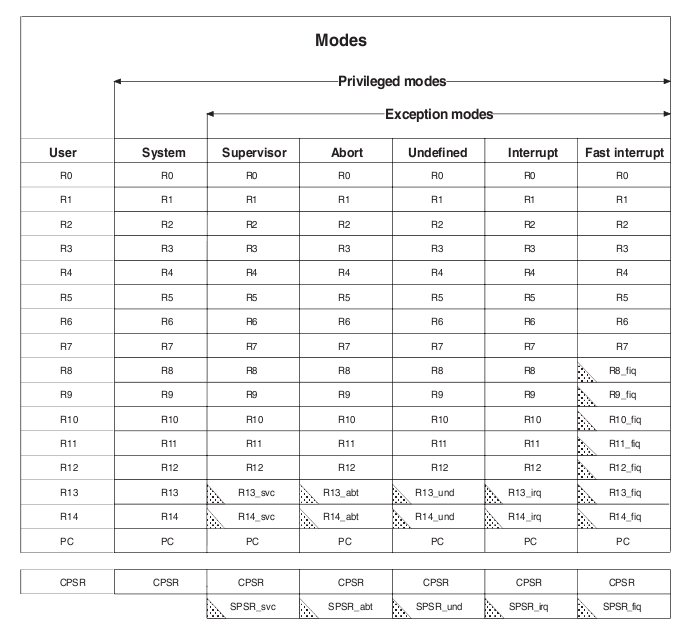
\includegraphics[scale=0.5]{img/registros}

\caption{\label{fig:registros}Registros del procesador}



\end{figure}



\section{Modelo de memoria}

Esta familia de procesadores soporta dos revisiones, procesadores
con MMU y procesadores sin MMU, en el caso de los que soportan MMU
podemos direccionar hasta 4 GB de memoria si tenemos el suficiente
espacio en disco y un sistema operativo que soporte el \emph{swapping}.

En otro caso podemos direccionar 2 GB de memoria (aunque sólo una
pequeña parte de esta memoria estaría físicamente mapeada a algún
dispositivo), y los otros 2 GB están mapeados a la configuración de
los dispositivos externos del microprocesador.

En la figura \ref{Flo:memoria} se muestran las regiones de memoria
mapeadas a ciertos dispositivos externos del microprocesador. En este
ejemplo escribir en la dirección \emph{0x000FFFF} equivale algún comando
al dispositivo USART.

La distribución de la memoria depende del fabricante, es aquí donde
entra en juego el desarrollo de un simulador, como se detalla en el
capítulo \ref{ch:simulador_arm}.

%
\begin{figure}[!h]
\centering{}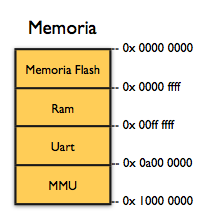
\includegraphics[scale=0.5]{img/memoria}\caption{Modelo de memoria en ARM}
\label{Flo:memoria}
\end{figure}



\section{Formato de las instrucciones}

Los microcontroladores y microprocesadores \ac{ARM}, dependiendo
del estándar que sigan, pueden soportar tres conjuntos de instrucciones:
\begin{itemize}
\item \emph{ARM.} Conjunto de instrucciones RISC de 32 bits, puede direccionar
hasta 4 GB de memoria. Cualquier microprocesador o microcontrolador
\ac{ARM} soporta este modo.
\item \emph{Thumb}. Conjunto de instrucciones RISC de 16 bits (aunque las
revisiones actuales soportan tamaños variables para algunas instrucciones,
pudiendo ser de 16 o 32 bis), trabaja bajo la premisa de generar código
más compacto, sin embargo tiene la limitación de que solo puede direccionar
hasta 64K de memoria. Funciona bien para microcontroladores con menos
capacidad.
\item \emph{Jazelle}. Este conjunto de instrucciones está diseñado para
soportar el bytecode de Java a nivel de hardware, sin embargo este
conjunto de instrucciones no se ha consolidado entre otras razones
porque es requerido soporte de software para hacerlo. 
\end{itemize}
En este trabajo utilizamos las instrucciones ARM, posteriormente es
posible extender el trabajo a instrucciones de Thumb y Jazelle.


